%%%%%%%%%%%%%%%%%%%%%%%%%%%%%%%%%%%%%%%%%%%%%%%%%%%%%%%%%%%%%%%%%%%%%%%%%%%%%%%%
%%%%%%%%%%%%%%%%%%%%%%%%%%%%%%%%%%%%%%%%%%%%%%%%%%%%%%%%%%%%%%%%%%%%%%%%%%%%%%%%
%%% Template for AIMS Rwanda Assignments         %%%              %%%
%%% Author:   AIMS Rwanda tutors                             %%%   ###        %%%
%%% Email: tutors2017-18@aims.ac.rw                               %%%   ###        %%%
%%% Copyright: This template was designed to be used for    %%% #######      %%%
%%% the assignments at AIMS Rwanda during the academic year %%%   ###        %%%
%%% 2017-2018.                                              %%%   #########  %%%
%%% You are free to alter any part of this document for     %%%   ###   ###  %%%
%%% yourself and for distribution.                          %%%   ###   ###  %%%
%%%                                                         %%%              %%%
%%%%%%%%%%%%%%%%%%%%%%%%%%%%%%%%%%%%%%%%%%%%%%%%%%%%%%%%%%%%%%%%%%%%%%%%%%%%%%%%
%%%%%%%%%%%%%%%%%%%%%%%%%%%%%%%%%%%%%%%%%%%%%%%%%%%%%%%%%%%%%%%%%%%%%%%%%%%%%%%%


%%%%%% Ensure that you do not write the questions before each of the solutions because it is not necessary. %%%%%% 

\documentclass[12pt,a4paper]{article}

%%%%%%%%%%%%%%%%%%%%%%%%% packages %%%%%%%%%%%%%%%%%%%%%%%%
\usepackage{amsmath}
\usepackage{amssymb}
\usepackage{amsthm}
\usepackage{amsfonts}
\usepackage{graphicx}
\usepackage[all]{xy}
\usepackage{tikz}
\usepackage{verbatim}
\usepackage{float}
\usepackage[left=2cm,right=2cm,top=3cm,bottom=2.5cm]{geometry}
\usepackage{hyperref}
\usepackage{caption}
\usepackage{subcaption}
\usepackage{psfrag}
\usepackage{mathrsfs}
\usepackage{actuarialangle}
\usepackage[T1]{fontenc}
\usepackage{float}
%%%%%%%%%%%%%%%%%%%%% students data %%%%%%%%%%%%%%%%%%%%%%%%
\newcommand{\student}{Yusuf Brima}
\newcommand{\course}{Fluid Mechanics}
\newcommand{\assignment}{2}

%%%%%%%%%%%%%%%%%%% using theorem style %%%%%%%%%%%%%%%%%%%%
\newtheorem{thm}{Theorem}
\newtheorem{lem}[thm]{Lemma}
\newtheorem{defn}[thm]{Definition}
\newtheorem{exa}[thm]{Example}
\newtheorem{rem}[thm]{Remark}
\newtheorem{coro}[thm]{Corollary}
\newtheorem{quest}{Question}[section]

%%%%%%%%%%%%%%  Shortcut for usual set of numbers  %%%%%%%%%%%

\newcommand{\N}{\mathbb{N}}
\newcommand{\Z}{\mathbb{Z}}
\newcommand{\Q}{\mathbb{Q}}
\newcommand{\R}{\mathbb{R}}
\newcommand{\C}{\mathbb{C}}

%%%%%%%%%%%%%%%%%%%%%%%%%%%%%%%%%%%%%%%%%%%%%%%%%%%%%%%555
\begin{document}

%%%%%%%%%%%%%%%%%%%%%%% title page %%%%%%%%%%%%%%%%%%%%%%%%%%
\thispagestyle{empty}
%\begin{figure}
%    \centering
%    \includegraphics[width=\textwidth]{aims_rwanda.jpg}
%\end{figure}
\begin{center}
\textbf{AFRICAN INSTITUTE FOR MATHEMATICAL SCIENCES \\[0.5cm]
(AIMS RWANDA, KIGALI)}
\vspace{1.0cm}
\end{center}

%%%%%%%%%%%%%%%%%%%%% assignment information %%%%%%%%%%%%%%%%
\noindent
\rule{17cm}{0.2cm}\\[0.3cm]
Name: \student \hfill Assignment Number: \assignment\\[0.1cm]
Course: \course \hfill Date: \today\\
\rule{17cm}{0.05cm}
\vspace{1.0cm}
\section*{Exercise 1}

\begin{enumerate}
		\item[(i)] Given the dynamical systems in \eqref{eq:1}, the $4^{th}$ order Runge-Kutta solution is plotted below.
				\begin{equation}
						  \frac{d\mathbf{x}}{dt} =  \begin{pmatrix}
		  								5 &  1\\
		  								3 & 1
		  						\end{pmatrix} \mathbf{x}
						\label{eq:1}
			  \end{equation}
					\begin{figure}[!h]
									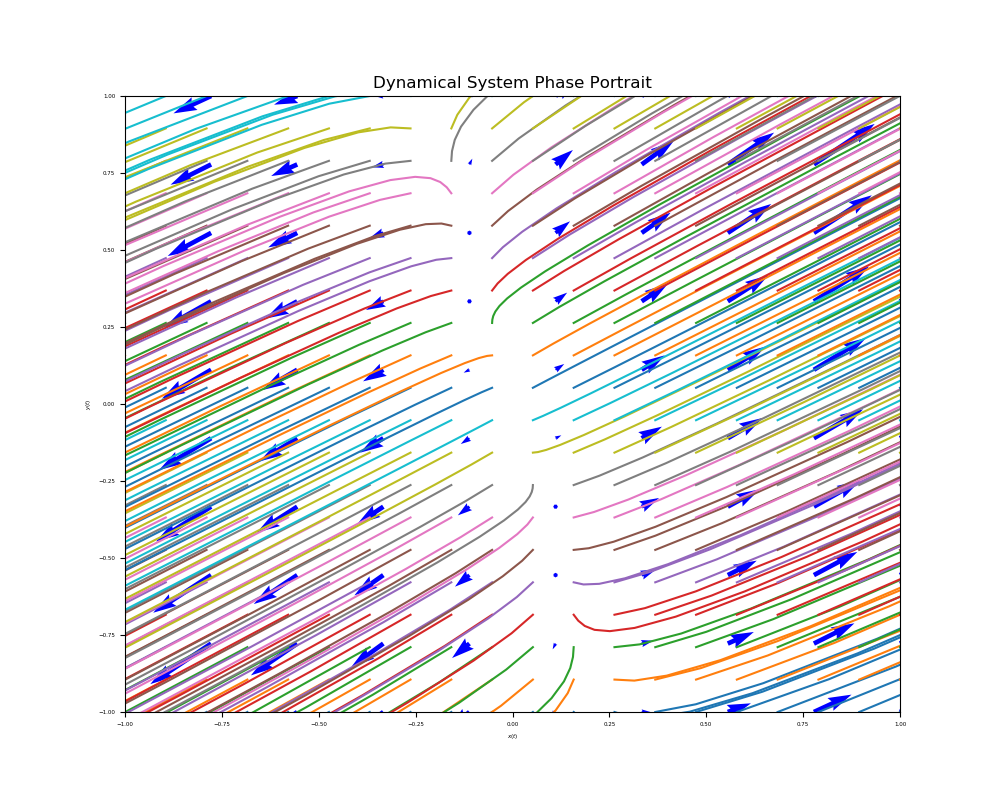
\includegraphics[width=480pt,  height=260pt]{./graphics/q001_a.png}
										\caption{A plot of the dynamical system of ODEs using RK4 method}
										\label{fig:q1}
								\end{figure}
					\item[(ii)] Given the dynamical systems in \eqref{eq:2}, the $4^{th}$ order Runge-Kutta solution is plotted below.
				\begin{equation}
						  \frac{d\mathbf{x}}{dt} =  \begin{pmatrix}
		  								2 &  -5\\
		  								1  & -2
		  						\end{pmatrix} \mathbf{x}
						\label{eq:2}
			  \end{equation}
					\begin{figure}[!h]
									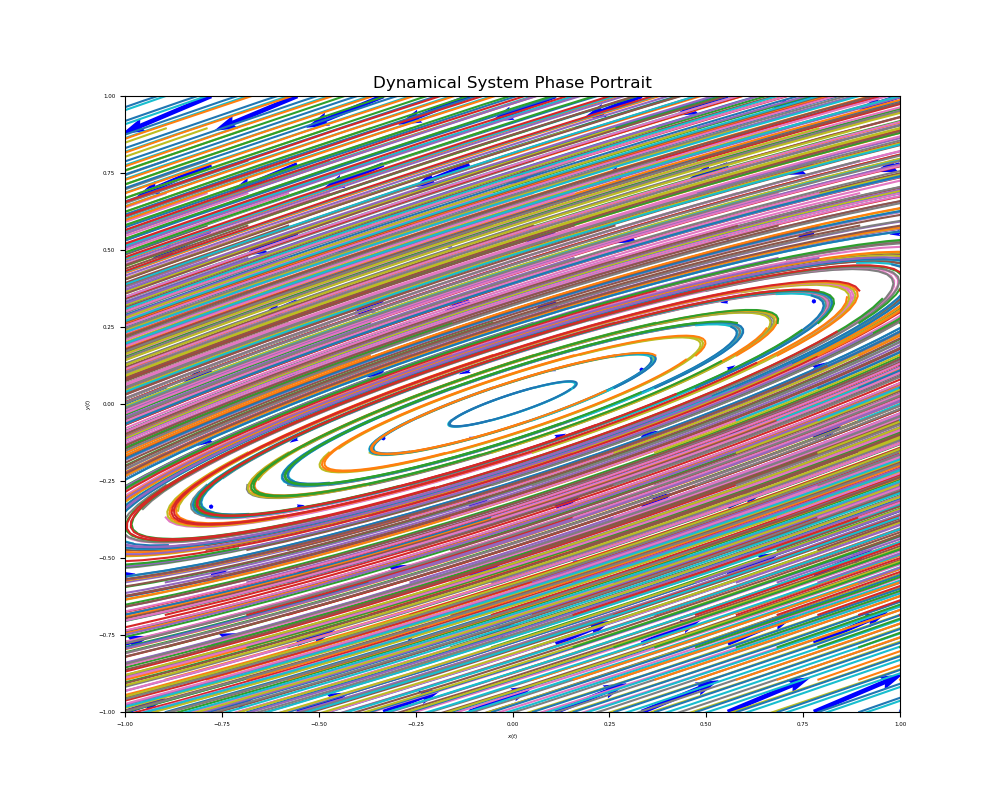
\includegraphics[width=480pt,  height=240pt]{./graphics/q001_b.png}
										\caption{A plot of the dynamical system of ODEs using RK4 method}
										\label{fig:q2}
								\end{figure}
					\item[(iii)] Given the dynamical systems in \eqref{eq:3}, the $4^{th}$ order Runge-Kutta solution is plotted below.
				\begin{equation}
						  \frac{d\mathbf{x}}{dt} =  \begin{pmatrix}
		  								1 &  -5\\
		  								1 & -3
		  						\end{pmatrix} \mathbf{x}
						\label{eq:3}
			  \end{equation}
					\begin{figure}[!h]
									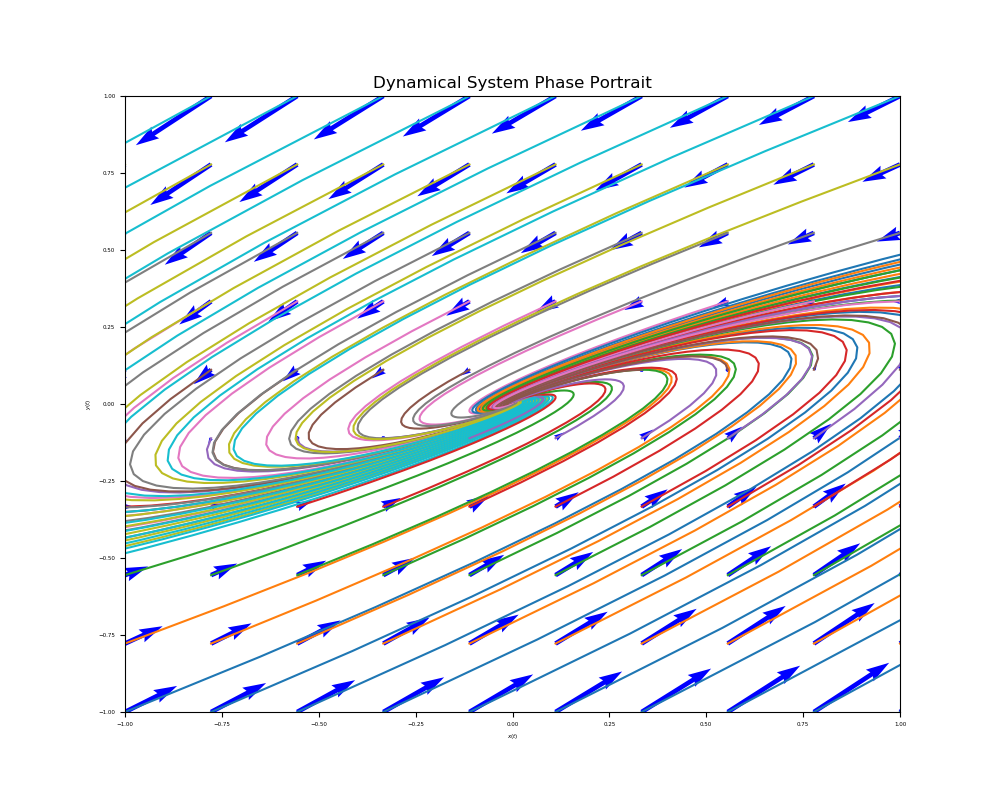
\includegraphics[width=480pt,  height=240pt]{./graphics/q001_c.png}
										\caption{A plot of the dynamical system of ODEs using RK4 method}
										\label{fig:q3}
								\end{figure}
								\item[(iv)] Given the dynamical systems in \eqref{eq:4}, the $4^{th}$ order Runge-Kutta solution is plotted below.
				\begin{equation}
						  \frac{d\mathbf{x}}{dt} =  \begin{pmatrix}
		  								2 &  -1\\
		  								 3 &  -2
		  						\end{pmatrix} \mathbf{x}
						\label{eq:4}
			  \end{equation}
					\begin{figure}[!h]
									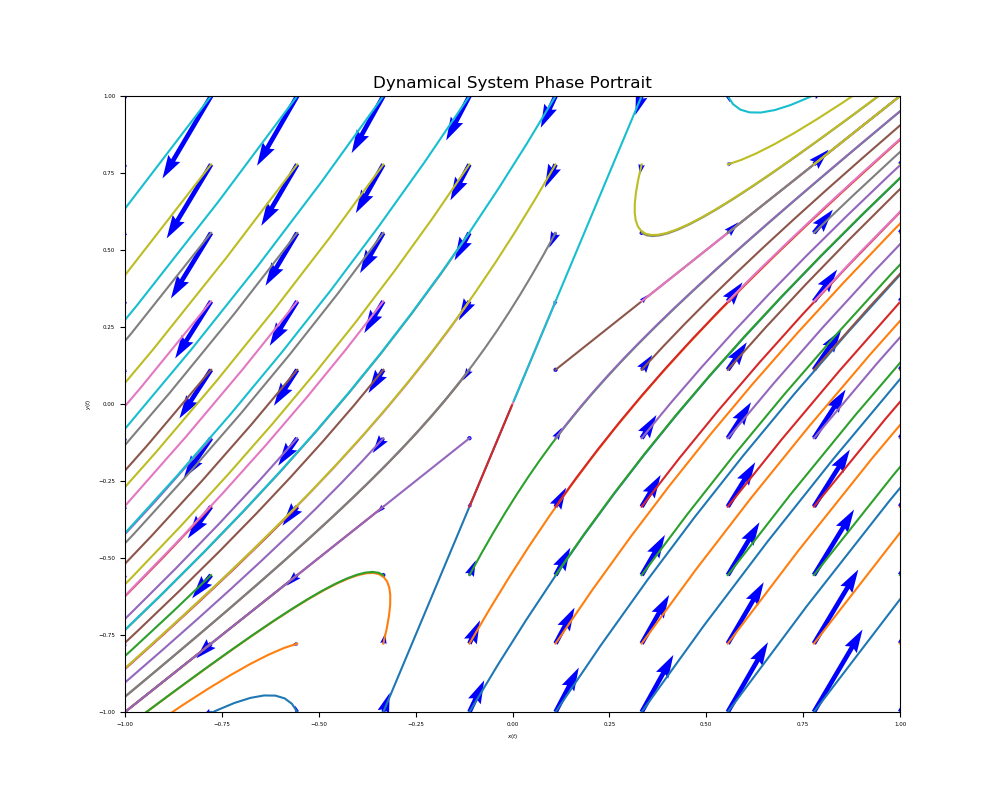
\includegraphics[width=500pt,  height=290pt]{./graphics/q001_d.png}
										\caption{A plot of the dynamical system of ODEs using RK4 method}
										\label{fig:q4}
								\end{figure}
\end{enumerate}
\section*{Exercise 2}
Given 
\begin{equation}
		\frac{dx}{dt} =  y - x^2, \quad
		\frac{dy}{dt} = x -2
		\label{eq:5}
\end{equation}
\begin{enumerate}
							\item[(i)]   We calculate the equilibrium point as thus:
								\begin{eqnarray}
										\label{eq:6}
										\frac{dx}{dt}  &=  y - x^2 \\
										\label{eq:7}
										\frac{dy}{dt}  &= x -2
								\end{eqnarray}
								To derive the equilibrium point of the above system,  we set it equal to 0 as indicated below.
							\begin{align*}
										\frac{dx}{dt}  &=  y - x^2 = 0 \\
									   \frac{dy}{dt}  &= x -2  = 0
								\end{align*}
								\begin{align*}
								       y - x^2 &= 0 \quad \implies x  = 2 \\
									   x -2  &= 0 \quad y = 4
								\end{align*}
								Thus the equilibrium points of the system is:
								\begin{align*}
										\begin{pmatrix}
												x_0 \\
												y_0
										\end{pmatrix}  &= \begin{pmatrix}
												2\\
												4
										\end{pmatrix}
								\end{align*}
							\item[(ii)]We proceed as follows to linearize the dynamical system around the equilibrium in \eqref{eq:5}.
							\begin{align*}
									-cy + dxy  &= 0\\
									y(-c + dx) &=  0 \quad \text{we divied through by }  y\\ 
									-c + + dx  &= 0\\
									dx  &=  x\\
									\therefore x &= \frac{c}{d}
							\end{align*}
									Let
\begin{equation}
 f_1= y-x^2       \label{c4}
\end{equation}
and

\begin{equation}
 f_2= x-2         \label{c5}
\end{equation}
Taking a partial derivative of \ref{c4} and \ref{c5} w. r. t. $x$ and $y$

 \(
   B=
	\begin{pmatrix}
			   \frac{\partial f_1}{\partial x} & \frac{\partial f_1}{\partial y} \\\\
               \frac{\partial f_2}{\partial x} & \frac{\partial f_2}{\partial y} \\
	\end{pmatrix}
\)

and substitute in the matrix to get,
\begin{equation}
B=
  \begin{pmatrix}
    {\begin{array}{cc}
   -2x & 1 \\
   1 & 0 \\
  \end{array} }\end{pmatrix} \label{c6}
\end{equation}

solving the matrix (\ref{c6}) at (2,4), we have:

\begin{equation}
B=
   \begin{pmatrix}
   		{\begin{array}{cc}
   			-4 & 1 \\
  			 1 & 0 \\
 			 \end{array} }
   \end{pmatrix}
\end{equation}


\begin{equation}
\bigg(\begin{smallmatrix}\frac{d x}{dt}  \\\\\frac{d y}{dt}  \end{smallmatrix}\bigg)= \begin{pmatrix} {\begin{array}{cc}
   -4 & 1 \\
   1 & 0 \\
  \end{array} } \end{pmatrix} \bigg(\begin{smallmatrix} x \\\\y \end{smallmatrix}\bigg)  
\end{equation}
Hence shown.
							\item[(iii)] We find the eigenvalue and eigenvector of the linearized system,  and the character of the equilibrium.
	
	 We are required to find Eigenvalues using the matrix we have found.

\begin{equation}
B=
  \left[ {\begin{array}{cc}
   -4 & 1 \\
   1 & 0 \\
  \end{array} } \right]
\end{equation}


\begin{equation}
\lambda^2 - tr(B)\lambda + det(B) =0  \label{c8}
\end{equation}
replacing for $tr(B)=-4$ and $ det(B)=-1$ in equation (\ref{c8}),

\begin{equation}
\lambda^2 + 4\lambda -1 =0  \label{c9}
\end{equation}
To find eigen values we solve (\ref{c9}) to get
\begin{eqnarray*}
\lambda_1 &=& \sqrt{5}-2  \\
\lambda_2 &=& -(2 + \sqrt{5})\\
\end{eqnarray*}

using  $(B- \lambda I)\vec{x} = 0$ to get eigenvector

if $\lambda_1 = \sqrt{5}-2 $:


\begin{equation}
 \begin{pmatrix}{\begin{array}{cc}
   -2-\sqrt{5} & 1 \\
   1 & 2 - \sqrt{5} \\
  \end{array} } \end{pmatrix}\bigg(\begin{smallmatrix} x \\\\y \end{smallmatrix}\bigg)= \bigg(\begin{smallmatrix} 0 \\\\ 0 \end{smallmatrix}\bigg)
\end{equation}

and
\begin{equation*}
( -2-\sqrt{5})x  + y = 0\Rightarrow y=( 2+ \sqrt{5})x.
\end{equation*}
Letting $x =\alpha$  so that $y=( 2+ \sqrt{5})\alpha $ and then

\begin{equation*}
v_1=\bigg(\begin{smallmatrix} x \\\\ y \end{smallmatrix}\bigg)=\alpha \bigg(\begin{smallmatrix} 1 \\\\  2+ \sqrt{5} \end{smallmatrix}\bigg)=\bigg(\begin{smallmatrix} 1 \\\\  2+ \sqrt{5} \end{smallmatrix}\bigg)
\end{equation*}
if $\alpha=1$





If $\lambda_1 = -(2 + \sqrt{5})$, we have



\begin{equation}
 \begin{pmatrix}  {\begin{array}{cc}
   -2+\sqrt{5} & 1 \\
   1 & 2 + \sqrt{5} \\
  \end{array} } \end{pmatrix}\bigg(\begin{smallmatrix} x \\\\y \end{smallmatrix}\bigg)= \bigg(\begin{smallmatrix} 0 \\\\ 0 \end{smallmatrix}\bigg)
\end{equation}

and
\begin{equation*}
( -2+\sqrt{5})x  + y = 0\Rightarrow y=( 2- \sqrt{5})x.
\end{equation*}
Letting $x =\alpha$  so that $y=( 2- \sqrt{5})\alpha $ and then

\begin{equation*}
v_2=\bigg(\begin{smallmatrix} x \\\\ y \end{smallmatrix}\bigg)=\alpha \bigg(\begin{smallmatrix} 1 \\\\  2- \sqrt{5} \end{smallmatrix}\bigg)=\bigg(\begin{smallmatrix} 1 \\\\  2- \sqrt{5} \end{smallmatrix}\bigg)
\end{equation*}
if $\alpha=1$


The general solution:
\[
  \begin{pmatrix} x(t)\\ y(t) \end{pmatrix}
  =C_1e^{\lambda_1 t}\vec{v_1} + C_2 e^{\lambda_2 t}\vec{v_2}    
\]

\[
  \begin{pmatrix} x(t)\\ y(t) \end{pmatrix}
  =C_1e^{(-2 + \sqrt{5}) t}\begin{pmatrix} 1 \\ 2+\sqrt{5} \end{pmatrix}  + C_2 e^{(-2 - \sqrt{5}) t}\begin{pmatrix} 1 \\ 2 - \sqrt{5} \end{pmatrix}    
\]


\begin{equation}
x(t)= C_1e^{(-2 + \sqrt{5})t}  + C_2e^{(-2 - \sqrt{5})t}    \label{c9}
\end{equation}
and
\begin{equation}
y(t)= C_1(2 + \sqrt{5})e^{(-2 + \sqrt{5})t} + C_2(2 - \sqrt{5})e^{(-2 - \sqrt{5})t}    \label{c10}
\end{equation}




It is a saddle point and equilibrium point stability is unstable.
							\item[(iv)] Given the dynamical systems above the $4^{th}$ order Runge-Kutta solution is plotted below.

					\begin{figure}[!h]
									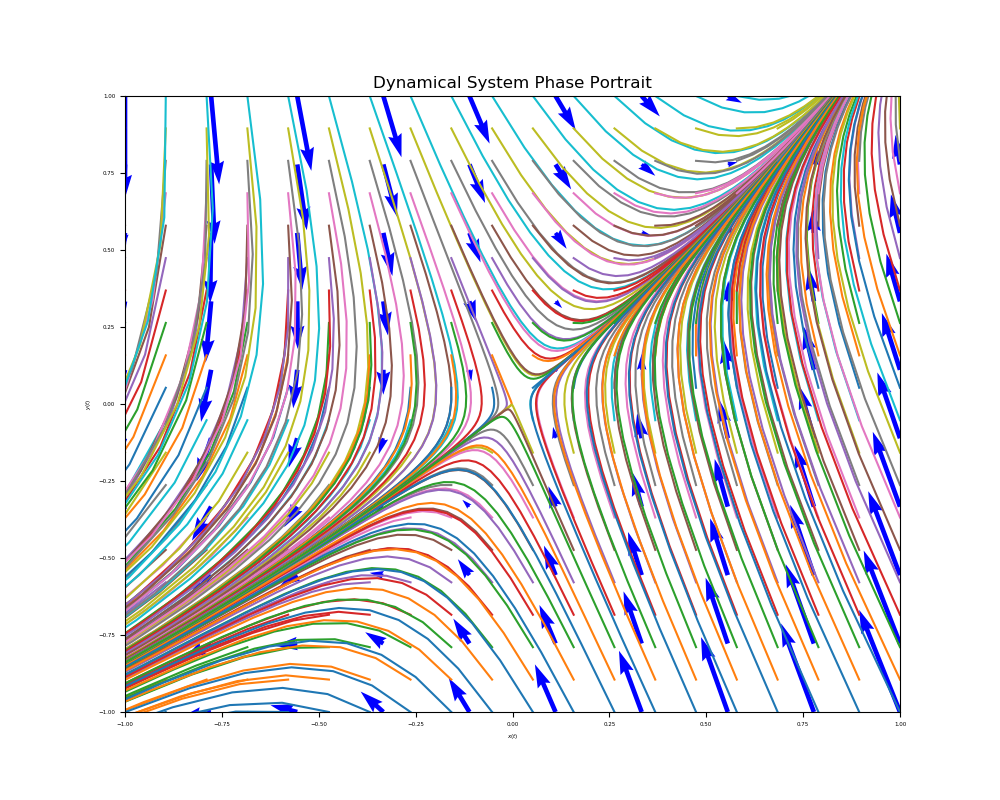
\includegraphics[width=430pt,  height=200pt]{./graphics/q002_a.png}
										\caption{A plot of the dynamical system of ODEs using RK4 method}
										\label{fig:q5}
								\end{figure}
\end{enumerate}

\end{document}